\documentclass[a4paper,11pt]{article}
\pdfoutput=1 % if your are submitting a pdflatex (i.e. if you have
             % images in pdf, png or jpg format)

\usepackage{jheppub} % for details on the use of the package, please
                     % see the JHEP-author-manual

\usepackage[T1]{fontenc} % if needed
\usepackage{kotex}
\usepackage{hhline}

\title{\boldmath HW5 - Emission line properties}


%% %simple case: 2 authors, same institution
%% \author{A. Uthor}
%% \author{and A. Nother Author}
%% \affiliation{Institution,\\Address, Country}

% more complex case: 4 authors, 3 institutions, 2 footnotes
\author{김태근, 윤한결, 강호철, 송진화}

% The "\note" macro will give a warning: "Ignoring empty anchor..."
% you can safely ignore it.

\affiliation{연세대학교 천문우주학과 F조}



\begin{document} 
\maketitle
\flushbottom

\section{BPT Diagram}
\label{sec:result}


\begin{figure}[h]
\centering
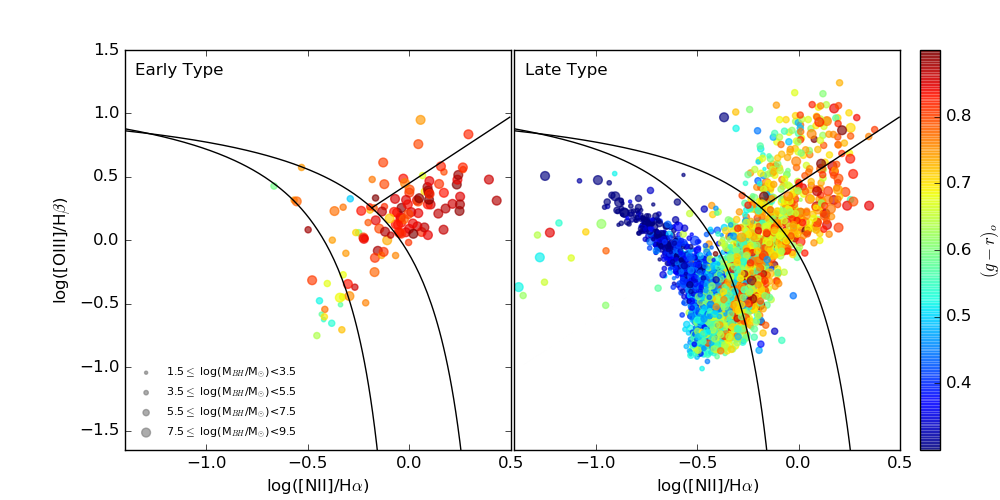
\includegraphics[height=60mm, width=100mm]{BPT.png}
\caption{\label{fig:i} BPT Diagram}
\end{figure}

OSSY database에서 추출한 데이터들을 이용해 Early-Type galaxies와 Late-Type galaxies로 구분한 후, 이를 이용해 BPT diagram을 그렸다. 붉게 표시된 은하일수록 redder한 은하이고 Early type이 주로 붉고 Late Type은 푸르다.
Early type galaxy들은 LINER 영역에 주로 분포되어 있고, Late type galaxy들은 모든 영역에 고루 분포하고 있는 것을 확인할 수 있다.
Early type은 상대적으로 온도가 낮고 붉은 별들을 많이 포함하고 있어 Ionization Nuclear Emission-line 방출량이 적으며, 이에 따라 LINER 영역에 몰려서 분포하게 된다고 유추해 볼 수 있다.
반면에 Late type은 Early type에 비해 star forming이 진행되는 비율이 높기 때문에 BPT diagram 상의 star forming 영역에 많은 수의 은하들이 분포하게 된다. 
우리의 그래프는 이러한 경향성과 Oh et al. 2013 논문과 유사한 결과를 보여준다고 볼 수 있다.

\section{Fraction of Early type's emission lines}

\begin{figure}[h]
\centering
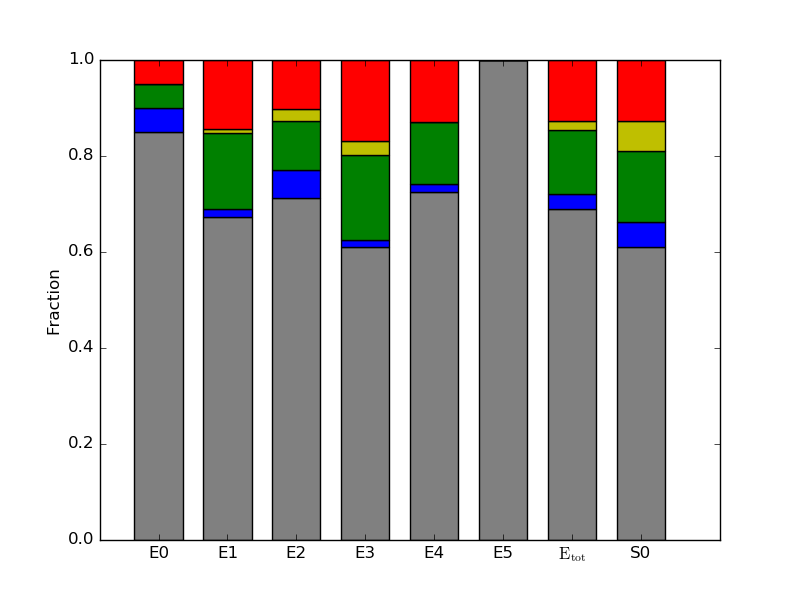
\includegraphics[height=60mm, width=100mm]{Earlybar.png}
\caption{\label{fig:ii}  Fraction of early type galaxies according to their emission line }
\end{figure}

그림\ref{fig:ii}를 보면 E5를 제외하고는 각각의 morphology type마다 어느 정도 비율의 차이는 존재하나 거의 비슷한 양상을 하고 있음을 확인할 수 있다.
Early type의 경우 Later type과 비교했을 때 무엇보다 weak emission line의 비율이 매우 높고, star forming이 매우 약해진 것이 바로 보이는데, 이는 각각의 Spiral에서 Elliptical로 가면서 star forming이 줄어들고 
AGN(Active Galactic Nucleus)이 힘을 잃어 radiation의 방출이 약해지는 것으로 해석할 수 있다. AGN의 약화로 인한 현상은 LINER(Low Ionization Nuclear Emission line Resion)의 약화로도 설명이 가능한데,
AGN의 활동 정도에 따라 약하게 이온화된 가스들에서 나오는 방출선이 줄어드는 것으로 Spiral에서 Elliptical 사이의 변화를 추론해 볼 수 있다.

Spiral에서 Elliptical의 진화방향을 따라가면, 위와 같은 흐름을 확인할 수 있었다. 이번에는 Elliptical의 경우만 생각해보자.
급격한 변화양상을 보이는 Spiral과는 다르게 Elliptical의 경우는 7번째 자료인 total 값과 나머지를 비교하여 보아도 큰 차이가 없는 것처럼 눈에 보이는 확실한 차이는 없다.
이는 은하의 morphology가 Elliptical로 들어서면서 더이상의 변화가 없어졌다는 해석이 되고, 이는 Spiral과 가장 큰 차이인 Star forming에서 근거를 찾을 수 있다.
이해를 돕기 위해 S0의 모습과도 비교했는데, 결국 Spiral에서 Elliptical로 진화가 되어가며 Star forming과 AGN이 힘을 잃어가며 진화가 멈추어감을 생각할 수 있다.

결국 Early type은 Elliptical만의 morphology에 대해서 각 형태별로 특별한 작용이나 진화단계에 있는 것이 아닌 단순히 Spiral에서 진화한 단계로 이심률의 차이만 있는 것으로 해석되며 Early type 내의 진화 방향은 보이지 않음을 확인할 수 있다.

\newpage

\section{Fraction of Late type's emission lines}


\begin{figure}[h]
\centering
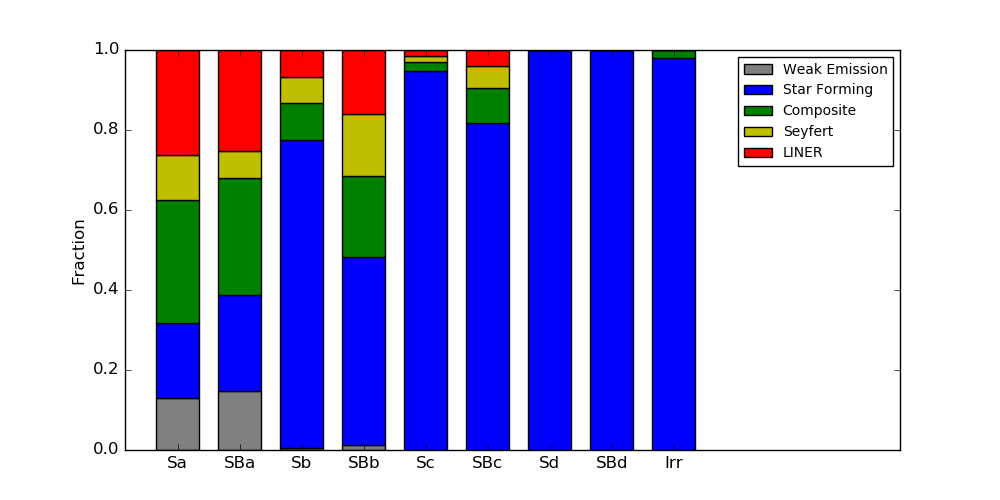
\includegraphics[height=60mm, width=100 mm]{Latebar.png}
\caption{\label{fig:iii} Fraction of late type galaxies according to their emission line }
\end{figure}


그림 \ref{fig:iii} 을 보면 Early type을 봤을 때와는 다르게 각각의 morphology type마다 뚜렷한 양상을 보여준다는 것을 알 수 있다. 
특히 바로 눈에 띄는 것은 Star forming으로서 우리가 알고 있는 바와 같이 Sd로 갈수록 Star forming이 강해지고 Sa 등은 Star forming이 Sd에 비하여 낮다는 결과가 나왔다.
좀 더 자세히 살펴보면 SBb나 SBc보다 Sb와 Sc가 좀 더 Star forming 이 많은 것도 알 수 있다. 따라서 SF 만 봐도 어느 정도 우리의 상식과 부합하는 것을 알 수 있다. 
다음으로 특징있는 것은 weak emission line인데 이는 그림 \ref{fig:ii}와 비교해보면 그 차이를 실감할 수 있다. 보통 Spiral의 가운데에는 SMBH가 있을 것이라 생각하고
따라서 AGN이 Elliptical보다 강력한 Radiation을 방출할 것이고 따라서 weak emission line은 Late type에는 거의 나타나지 않고 Early type 혹은 Lenticula에 많이 나타나는 것을 볼 수 있다.
마지막으로 LINER도 Sd에 가까이 갈수록 줄어드는 것을 확인할 수 있는데 줄어드는 것도 명확히 줄어드는 것이 아니며 그림 \ref{fig:ii} 에서 보다시피 다들 어느 정도 LINER를 갖고 있지만 규칙성을 찾기 힘든 상황이다.
실제로도 이렇게 넓은 범위에서 관측되는 성질 때문에 천문학자들 간에도 꽤 논쟁이 있다고 한다. 그래프로 알 수 있는 것은 그저 Sd, SBd, Irregular에서는 LINER가 없으며 Spiral에서는 대개 Bulge가 커질수록,
Bar가 있을 수록 좀 더 크게 관측된다는 것 정도이다. 마찬가지로 Seyfert 역시 전체적인 경향은 d로 갈수록 줄어들지만 규칙성을 찾기가 까다롭다.


\end{document}
